%--------------------- Goals -----------------------------------
\begin{frame}[c]{Problem statement}
 \begin{center}
	{\Large How to recover from intrusions in PaaS?}
	\end{center}
	\note{
	Assim sendo, como podemos recuperar das intrusões?
	}
\end{frame}

%-----------------------------------------
\section{Related Work}
\begin{frame}[t]{Goals}
      \vskip-0.5cm
      \textbf{Accept intrusions and remove their effects}
      \vskip0.5cm
		\begin{itemize}
			\item Identify the intrusion effects
			\item Remove intrusion effects
			\item Recover the application integrity
			\item Tolerate intrusions: recovery without exposing downtime	\footnote{Does not replace the prevention and tolerance}

			\item Recover from user and administrator mistakes
		\end{itemize}
		\note{
		Ou seja, como podemos aceitar intrusões e remover os seus efeitos? O ideal seria conseguir determinar quais foram os efeitos da intrusão, remove-los e recuperar a integridade da aplicação. Como extra, se conseguissemos fazer isto sem que a aplicação se torne indisponível para os utilizadores, então teriamos um sistema tolerante a intrusões. Como extra, também poderiamos recuperar de erros dos utilizadores e administradores. São exactamente estes os objectivos dos serviços recuperação de intrusões. Vejamos como é o processo de recuperação nos sistemas actuais.
		}
\end{frame}


%---------------------Related Work-----------------------------------
\begin{frame}[t]{1. Identification of intrusion effects}
  \textbf{Goal:} Identify the intrusion actions or objects
  \vspace{2ex}
  \begin{itemize}
    \item IDS: {\footnotesize \textit{[Taser,ITDB,Phoenix,Retro,Dare,Goel et al., Undo for Operators]}}
    \item Software update {\footnotesize \textit{[Warp,Aire]}} 
  \end{itemize}
    
\note{
O processo de recuperação começa após o administrador determinar um conjunto de dados ou acções que foram afectados. Os administradores podem ser apoiados por sistemas de detecção a intrusões. Em alternativa, podem realizar um update ao software da aplicação para resolver uma vulnerabilidade.
} 
\end{frame}


%------------------------------

\begin{frame}[c]{1. Identification of intrusion effects}
	\begin{center}
		\begin{figure} 
			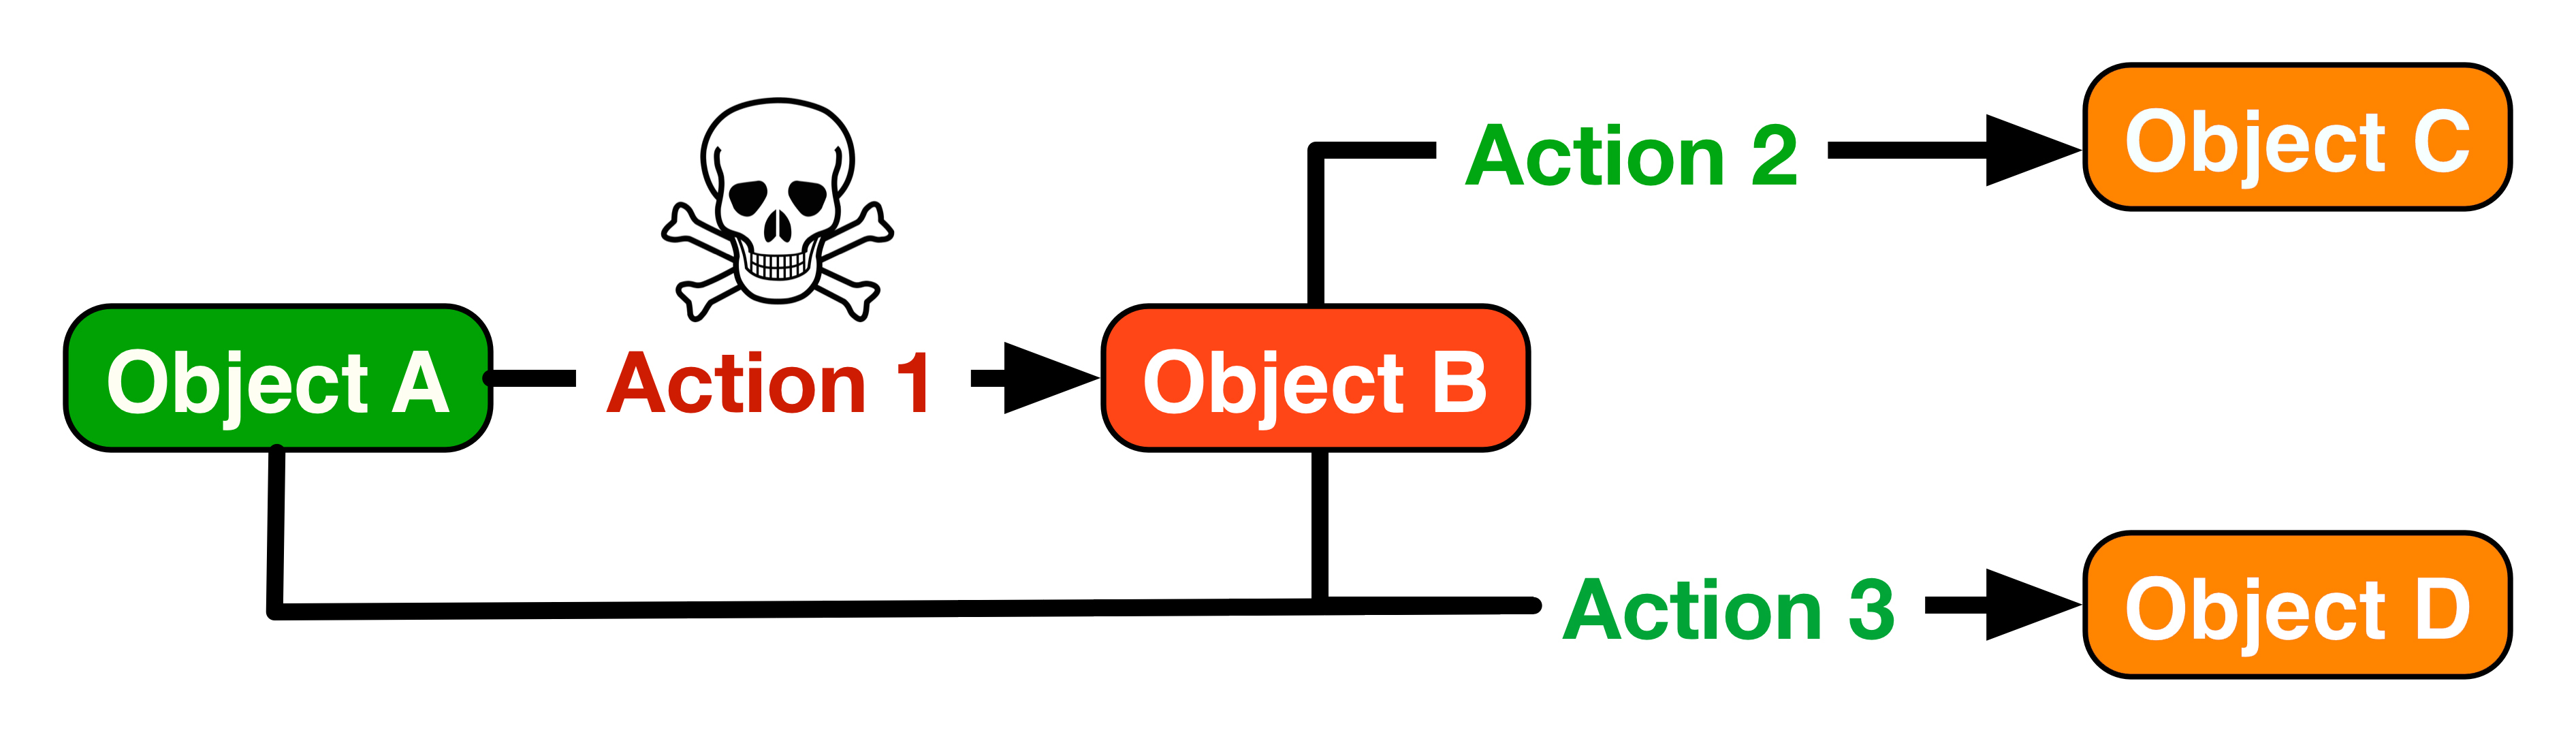
\includegraphics[width=0.8\textwidth]{img/propagation}
			\end{figure}
	\end{center}
\note{
Partindo dos dados fornecidos pelo administrador, os serviços de recuperação determinam quais os objectos e pedidos  afectados. 
Ou seja, se criarmos um grafo em que os nós são objectos e os vertices são as acções que lêem um objecto e escrevem outro, verificamos que as acções são interdependentes através dos objectos. 
Por exemplo, se acção 1 foi um ataque, então o objecto B foi afectado. Por isso, remover os efeitos da intrusão implica remover o valor que a acção 1 escreveu no objecto B.
} 
\end{frame}

%------------------------------


\begin{frame}[t]{2. Remove intrusion effects}
		\begin{itemize}
	\item Versioning {\footnotesize \textit{[Phoenix, Warp,Aire]}}
	\item Snapshot {\footnotesize \textit{[Taser, Retro,Date, Undo for Operators]}}
	\item Compensation {\footnotesize \textit{[Goel et al,ITDB]}}
		\end{itemize}
		\vskip1cm
		\begin{center}
		  \textbf{storage vs computing}
		\end{center}
		\note{
		Existem 3 alternativas para remover os efeitos:
		- Podemos carregar a versão do objecto imediatamente anterior ao ataque.
		- Podemos carregar um snapshot do sistema e refazer as operações legitimas até ao momento da intrusão
		- Ou então inverter todas as acções realizadas sobre o objecto desde o momento presente até ao momento anterior à intrusão.

		Cada uma destas propostas tem vantagens e desvantagens. De cima para baixo, ordenadas pelo espaço ocupado em disco e de baixo para cima ordenadas pelo número de acções que temos de repetir para um valor.
		}
\end{frame}


%----------------------------------------
\begin{frame}[t]{3. Recover the application integrity}
		\begin{center}
			\vskip-20pt
		\begin{figure} 
			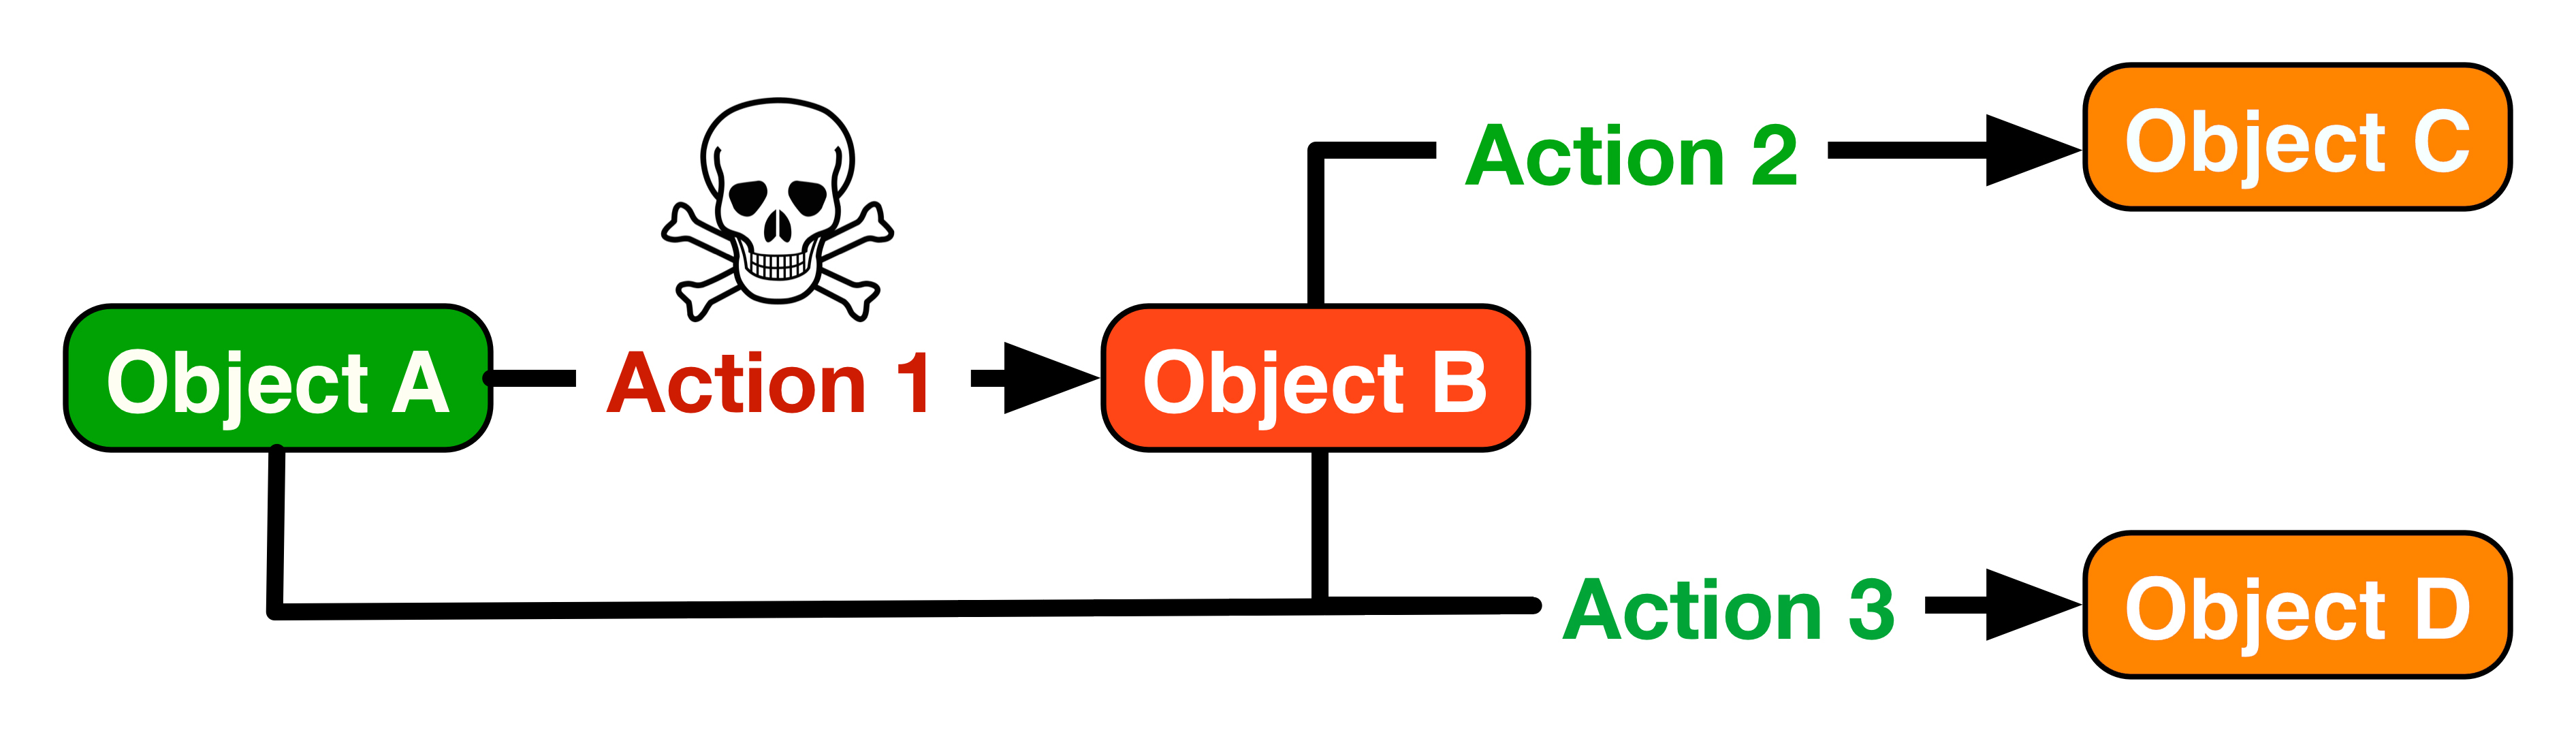
\includegraphics[width=0.8\textwidth]{img/propagation}
			\end{figure}
		\end{center}
	\begin{itemize}
		\item No replay {\footnotesize \textit{[Taser, ITDB, Phoenix]}}
		\item Taint via replay {\footnotesize \textit{[Retro,Dare,Goel et al,Warp,Aire]}}
		\item Replay all {\footnotesize \textit{[Undo for Operators]}}
	\end{itemize}

\note{
Vejamos agora o grafo de dependencias de novo. Mesmo que removamos o objecto B, o ataque continua a ter efeitos. Os objectos C e D foram influênciados, tainted, porque leram o valor errado do objecto B. Alguns dos projectos apresentados limitam-se a remover também os objectos C e D. Esta abordagem é insuficiente porque continua a penalizar os utilizadores legitimos.

Outros, removem apenas o valor do objecto B mas voltam a executar as acções 2 e 3 e caso os objectos C e D sejam agora diferentes, vão re-executar as acções que leiam destes objectos também. Este ciclo é recursivo. Neste caso, o sistema recupera um estado consistente e os utilizadores já não são penalizados.

No entanto, podem haver dependências indirectas que não são determinadas pelo grafo. Por isso, um dos trabalhos apresentados propõe realizar todos as acções legitimas. Neste caso, o sistema carrega uma cópia anterior à intrusão do objecto B e refaz as acções 2 e 3 e todas as seguintes, de modo ordenado.
} 
%marcar os tainted
\end{frame}

%-------------------------------------------------------------
\begin{frame}[t]{Recovery: Where?}
		\begin{itemize}
	\item Operating system {\footnotesize \textit{[Taser,Retro]}}:
	\begin{itemize}
			\item System calls, files and sockets
	\end{itemize}
	\item Database {\footnotesize \textit{[ITDB,Phoenix]}}:
	\begin{itemize}
		\item Read and write sets: table, table block, row or field
	\end{itemize}
	\item Web Applications{\footnotesize \textit{[Goel et al, Warp,Aire,Undo for Operators]}}:
		\begin{itemize}
		\item User requests and database transactions
		\end{itemize}
	\end{itemize}


\note{
O modo de estabelecer os vertices do grafo que definem as dependencias, depende da camada da aplicação que queremos recuperar. As propostas para File System Recovery baseiam-se em dependências estabelecidas pelas system calls realizadas pelos processos interligando objectos como os ficheiros e sockets. 
No caso das base de dados, as dependências são estabelecidas pelos valores que a transacção lê e escreve.
No caso da aplicação, que geralmente são suportadas por bases de dados, as dependências são estabelecidas não só pelas regras das bases de dados como também pela camada aplicacional. A camada aplicacional pode usar um transacção para gerar os valores da transação seguinte.
 } 
\end{frame}